\nwfilename{}\nwbegindocs{0}\nwenddocs{}\nwbegindocs{1}\nwdocspar% ===> this file was generated automatically by noweave --- better not edit it
\section*{Introduction}
The program \ty{plotLine} plots lines using the R-package
ggplot2~\cite{wic16:ggp}. It takes as input either two or three
columns of data. The first two columns are the x- and y-coordinates,
the optional third column is the group. Figure~\ref{fig:plot}A shows
some example data for two groups and Figure~\ref{fig:plot}B its plot.

\begin{figure}
  \begin{center}
    \begin{tabular}{cc}
        \textbf{A} & \textbf{B}\\
        \begin{tabular}{lll}
          0 & 0 & g1\\
          1 & 1 & g1\\
          2 & 2 & g1\\
          0 & 2 & g2\\
          2 & 4 & g2\\
          4 & 8 & g2
        \end{tabular}
        &
        \raisebox{1.5cm}{\rotatebox{-90}{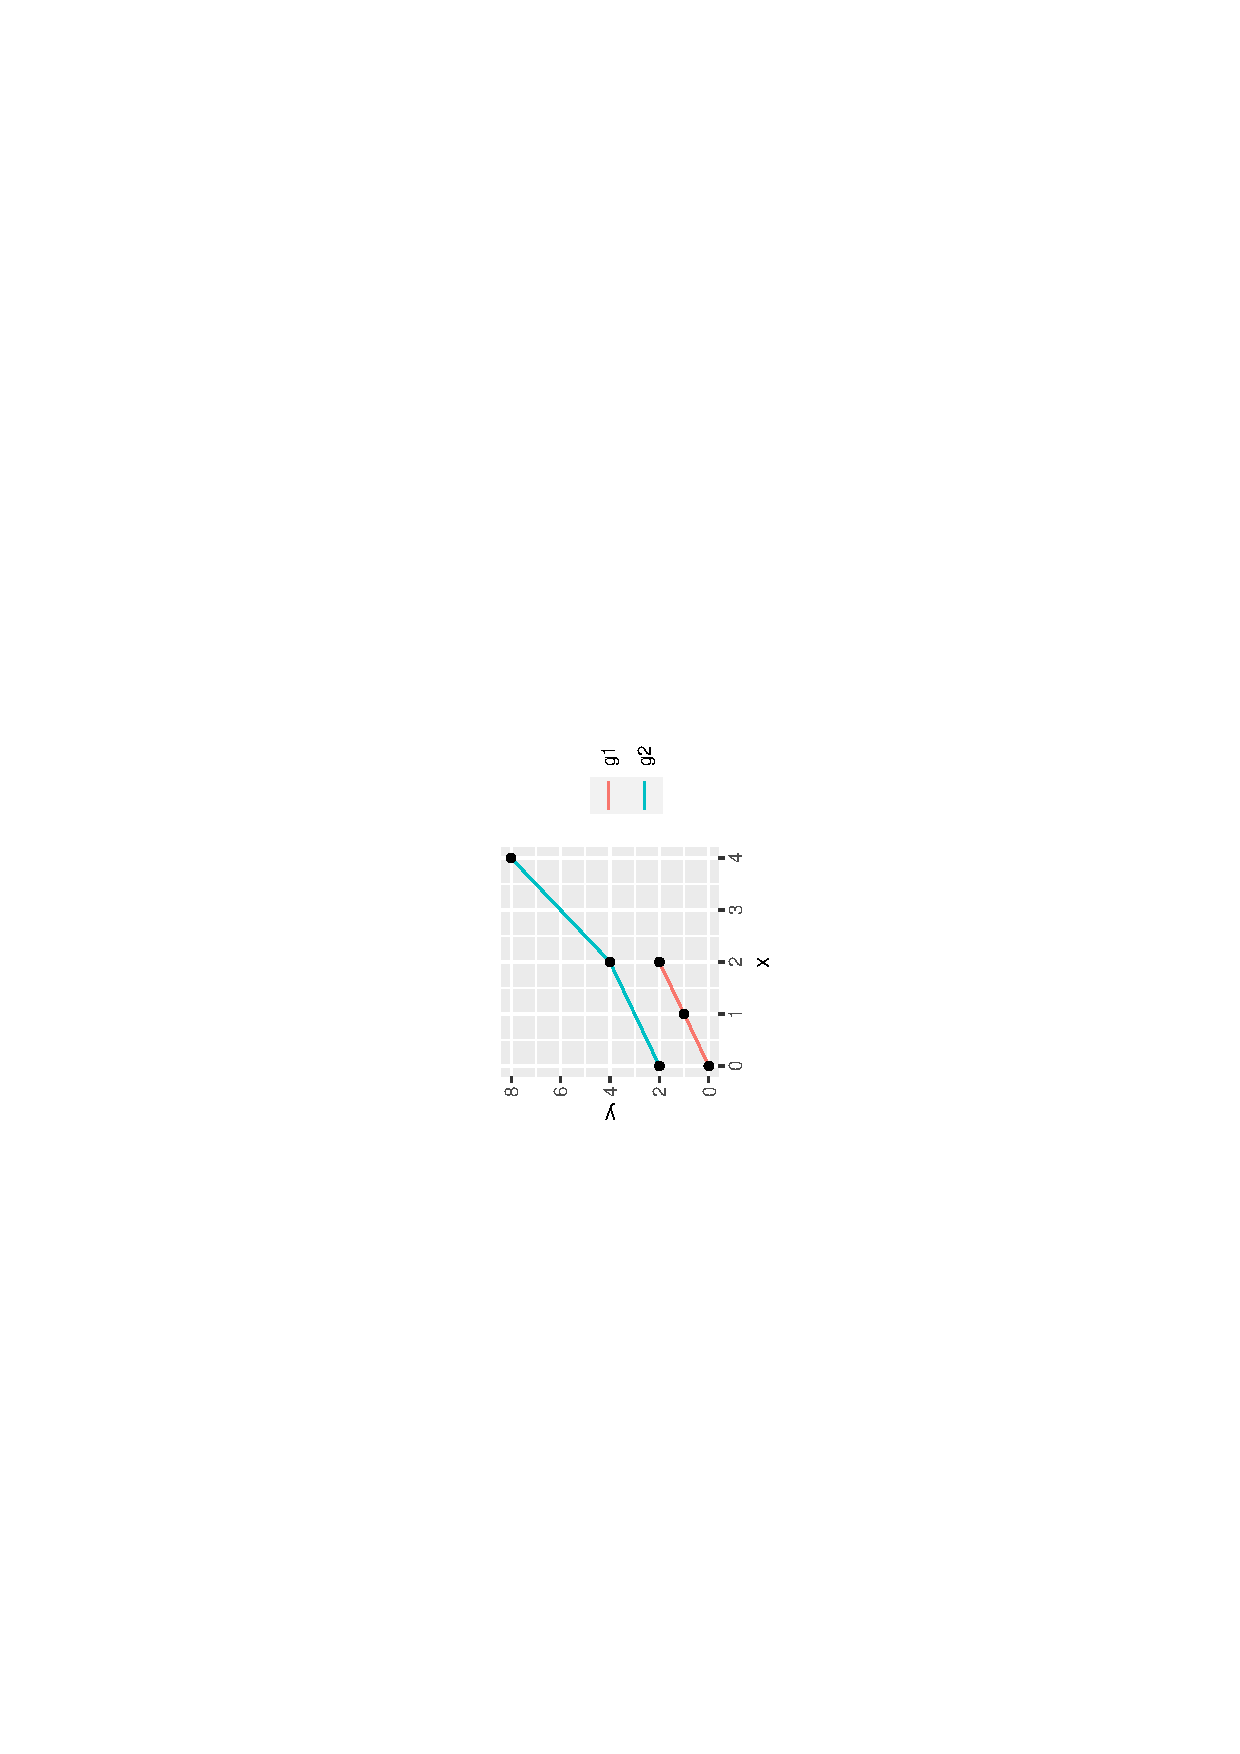
\includegraphics{plotLine}}}
    \end{tabular}
  \end{center}
  \caption{Example data (\textbf{A}) plotted with \ty{plotLine}
    (\textbf{B}).}\label{fig:plot}
\end{figure}

\section*{Implementation}
The outline of \ty{plotLine} has hooks for imports, types, functions,
and the logic of the main function.
\nwenddocs{}\nwbegincode{2}\sublabel{NW0-Xo4Ez-1}\nwmargintag{{\nwtagstyle{}\subpageref{NW0-Xo4Ez-1}}}\moddef{plotLine.go~{\nwtagstyle{}\subpageref{NW0-Xo4Ez-1}}}\endmoddef\nwstartdeflinemarkup\nwenddeflinemarkup
package main

import (
          \LA{}Imports, Ch.~\ref{ch:pl}~{\nwtagstyle{}\subpageref{NW0-2OMat3-1}}\RA{}
)
\LA{}Types, Ch.~\ref{ch:pl}~{\nwtagstyle{}\subpageref{NW0-HbCKE-1}}\RA{}
\LA{}Functions, Ch.~\ref{ch:pl}~{\nwtagstyle{}\subpageref{NW0-3njhFS-1}}\RA{}
func main() \{
          \LA{}Main function, Ch.~\ref{ch:pl}~{\nwtagstyle{}\subpageref{NW0-4WX4eM-1}}\RA{}
\}
\nwnotused{plotLine.go}\nwendcode{}\nwbegindocs{3}\nwdocspar
In the main function we set the usage, declare the options, parse the
options, and parse the input files.
\nwenddocs{}\nwbegincode{4}\sublabel{NW0-4WX4eM-1}\nwmargintag{{\nwtagstyle{}\subpageref{NW0-4WX4eM-1}}}\moddef{Main function, Ch.~\ref{ch:pl}~{\nwtagstyle{}\subpageref{NW0-4WX4eM-1}}}\endmoddef\nwstartdeflinemarkup\nwusesondefline{\\{NW0-Xo4Ez-1}}\nwenddeflinemarkup
\LA{}Set usage, Ch.~\ref{ch:pl}~{\nwtagstyle{}\subpageref{NW0-z3Bve-1}}\RA{}
\LA{}Declare options, Ch.~\ref{ch:pl}~{\nwtagstyle{}\subpageref{NW0-22PPLz-1}}\RA{}
\LA{}Parse options, Ch.~\ref{ch:pl}~{\nwtagstyle{}\subpageref{NW0-1mk760-1}}\RA{}
\LA{}Parse input files, Ch.~\ref{ch:pl}~{\nwtagstyle{}\subpageref{NW0-3D30ZY-1}}\RA{}
\nwused{\\{NW0-Xo4Ez-1}}\nwendcode{}\nwbegindocs{5}\nwdocspar
The usage consists of the actual usage message, an explanation of the
program's purpose, and an example command.
\nwenddocs{}\nwbegincode{6}\sublabel{NW0-z3Bve-1}\nwmargintag{{\nwtagstyle{}\subpageref{NW0-z3Bve-1}}}\moddef{Set usage, Ch.~\ref{ch:pl}~{\nwtagstyle{}\subpageref{NW0-z3Bve-1}}}\endmoddef\nwstartdeflinemarkup\nwusesondefline{\\{NW0-4WX4eM-1}}\nwenddeflinemarkup
u := "plotLine [-h] [option]... [file]..."
p := "Plot lines from columns of x/y data " +
          "and an optional group column."
e := "plotLine -x Time -y [RNA] foo.dat"
clio.Usage(u, p, e)
\nwused{\\{NW0-4WX4eM-1}}\nwendcode{}\nwbegindocs{7}\nwdocspar
We import \ty{clio}.
\nwenddocs{}\nwbegincode{8}\sublabel{NW0-2OMat3-1}\nwmargintag{{\nwtagstyle{}\subpageref{NW0-2OMat3-1}}}\moddef{Imports, Ch.~\ref{ch:pl}~{\nwtagstyle{}\subpageref{NW0-2OMat3-1}}}\endmoddef\nwstartdeflinemarkup\nwusesondefline{\\{NW0-Xo4Ez-1}}\nwprevnextdefs{\relax}{NW0-2OMat3-2}\nwenddeflinemarkup
"github.com/evolbioinf/clio"
\nwalsodefined{\\{NW0-2OMat3-2}\\{NW0-2OMat3-3}\\{NW0-2OMat3-4}\\{NW0-2OMat3-5}\\{NW0-2OMat3-6}\\{NW0-2OMat3-7}\\{NW0-2OMat3-8}\\{NW0-2OMat3-9}\\{NW0-2OMat3-A}\\{NW0-2OMat3-B}\\{NW0-2OMat3-C}}\nwused{\\{NW0-Xo4Ez-1}}\nwendcode{}\nwbegindocs{9}\nwdocspar
Apart from the version, we declare options concerning the axes, the
plot type, the graphics device, and the underlying R script.
\nwenddocs{}\nwbegincode{10}\sublabel{NW0-22PPLz-1}\nwmargintag{{\nwtagstyle{}\subpageref{NW0-22PPLz-1}}}\moddef{Declare options, Ch.~\ref{ch:pl}~{\nwtagstyle{}\subpageref{NW0-22PPLz-1}}}\endmoddef\nwstartdeflinemarkup\nwusesondefline{\\{NW0-4WX4eM-1}}\nwenddeflinemarkup
var optV = flag.Bool("v", false, "print program version " +
          "and other information")
\LA{}Declare axes options, Ch~\ref{ch:pl}~{\nwtagstyle{}\subpageref{NW0-3Gh3I0-1}}\RA{}
\LA{}Declare plot type options, Ch.~\ref{ch:pl}~{\nwtagstyle{}\subpageref{NW0-2Xy0v1-1}}\RA{}
\LA{}Declare device options, Ch.~\ref{ch:pl}~{\nwtagstyle{}\subpageref{NW0-26XxAt-1}}\RA{}
\LA{}Declare script options, Ch.~\ref{ch:pl}~{\nwtagstyle{}\subpageref{NW0-1Duv4j-1}}\RA{}
\nwused{\\{NW0-4WX4eM-1}}\nwendcode{}\nwbegindocs{11}\nwdocspar
We import \ty{flag}.
\nwenddocs{}\nwbegincode{12}\sublabel{NW0-2OMat3-2}\nwmargintag{{\nwtagstyle{}\subpageref{NW0-2OMat3-2}}}\moddef{Imports, Ch.~\ref{ch:pl}~{\nwtagstyle{}\subpageref{NW0-2OMat3-1}}}\plusendmoddef\nwstartdeflinemarkup\nwusesondefline{\\{NW0-Xo4Ez-1}}\nwprevnextdefs{NW0-2OMat3-1}{NW0-2OMat3-3}\nwenddeflinemarkup
"flag"
\nwused{\\{NW0-Xo4Ez-1}}\nwendcode{}\nwbegindocs{13}\nwdocspar
The options for axes define their labels, the range, and the scale.
\nwenddocs{}\nwbegincode{14}\sublabel{NW0-3Gh3I0-1}\nwmargintag{{\nwtagstyle{}\subpageref{NW0-3Gh3I0-1}}}\moddef{Declare axes options, Ch~\ref{ch:pl}~{\nwtagstyle{}\subpageref{NW0-3Gh3I0-1}}}\endmoddef\nwstartdeflinemarkup\nwusesondefline{\\{NW0-22PPLz-1}}\nwenddeflinemarkup
var optX = flag.String("x", "x", "x-label")
var optY = flag.String("y", "y", "y-label")
var optXX = flag.String("X", "s:e", "x-range")
var optYY = flag.String("Y", "s:e", "y-range")
var optL = flag.String("l", "", "log-scale (x|y|xy)")
\nwused{\\{NW0-22PPLz-1}}\nwendcode{}\nwbegindocs{15}\nwdocspar
The user can set the base size of the plot, and opt for dots only or
lines with dots.
\nwenddocs{}\nwbegincode{16}\sublabel{NW0-2Xy0v1-1}\nwmargintag{{\nwtagstyle{}\subpageref{NW0-2Xy0v1-1}}}\moddef{Declare plot type options, Ch.~\ref{ch:pl}~{\nwtagstyle{}\subpageref{NW0-2Xy0v1-1}}}\endmoddef\nwstartdeflinemarkup\nwusesondefline{\\{NW0-22PPLz-1}}\nwenddeflinemarkup
var optS = flag.Int("s", 0, "base size")
var optD = flag.Bool("d", false, "dots only")
var optDD = flag.Bool("D", false, "dots with lines")
\nwused{\\{NW0-22PPLz-1}}\nwendcode{}\nwbegindocs{17}\nwdocspar
The user can set the graphical device, and set the width and height of
the plot it produces. Among the graphical devices supported by R, we
recognize five:
\begin{itemize}
\item postscript (p)
\item PDF (P)
\item x11 (x)
\item quartz (q)
\item windows (w)
\end{itemize}
\nwenddocs{}\nwbegincode{18}\sublabel{NW0-26XxAt-1}\nwmargintag{{\nwtagstyle{}\subpageref{NW0-26XxAt-1}}}\moddef{Declare device options, Ch.~\ref{ch:pl}~{\nwtagstyle{}\subpageref{NW0-26XxAt-1}}}\endmoddef\nwstartdeflinemarkup\nwusesondefline{\\{NW0-22PPLz-1}}\nwenddeflinemarkup
var optG = flag.String("g", "x", "graphical device, " +
          "first character of x11, ps, PDF, quartz, windows")
var optW = flag.Float64("w", 0.0, "width in cm")
var optHH = flag.Float64("H", 0.0, "height in cm")
\nwused{\\{NW0-22PPLz-1}}\nwendcode{}\nwbegindocs{19}\nwdocspar
The R script used for plotting is not accessible to the user. However,
the user can opt to have it printed to a file.
\nwenddocs{}\nwbegincode{20}\sublabel{NW0-1Duv4j-1}\nwmargintag{{\nwtagstyle{}\subpageref{NW0-1Duv4j-1}}}\moddef{Declare script options, Ch.~\ref{ch:pl}~{\nwtagstyle{}\subpageref{NW0-1Duv4j-1}}}\endmoddef\nwstartdeflinemarkup\nwusesondefline{\\{NW0-22PPLz-1}}\nwenddeflinemarkup
var optR = flag.String("r", "", "file for R script")
\nwused{\\{NW0-22PPLz-1}}\nwendcode{}\nwbegindocs{21}\nwdocspar
We parse the options and respond to \ty{-v}, as this might terminate
the program. Then we collect the values of options that are straight
forward in the variable \ty{args}. What remains are the more complex
options \ty{-X}, \ty{-Y}, \ty{-g}, and \ty{-l}. We respond to each one
of these in turn.
\nwenddocs{}\nwbegincode{22}\sublabel{NW0-1mk760-1}\nwmargintag{{\nwtagstyle{}\subpageref{NW0-1mk760-1}}}\moddef{Parse options, Ch.~\ref{ch:pl}~{\nwtagstyle{}\subpageref{NW0-1mk760-1}}}\endmoddef\nwstartdeflinemarkup\nwusesondefline{\\{NW0-4WX4eM-1}}\nwenddeflinemarkup
flag.Parse()
\LA{}Respond to \ty{-v}, Ch.~\ref{ch:pl}~{\nwtagstyle{}\subpageref{NW0-1Ge4wP-1}}\RA{}
args := new(Args)
\LA{}Collect option values, Ch.~\ref{ch:pl}~{\nwtagstyle{}\subpageref{NW0-45cVO7-1}}\RA{}
\LA{}Respond to \ty{-X}, Ch.~\ref{ch:pl}~{\nwtagstyle{}\subpageref{NW0-49jiXL-1}}\RA{}
\LA{}Respond to \ty{-Y}, Ch.~\ref{ch:pl}~{\nwtagstyle{}\subpageref{NW0-2jxkg3-1}}\RA{}
\LA{}Respond to \ty{-g}, Ch.~\ref{ch:pl}~{\nwtagstyle{}\subpageref{NW0-325APy-1}}\RA{}
\LA{}Respond to \ty{-l}, Ch.~\ref{ch:pl}~{\nwtagstyle{}\subpageref{NW0-1lVsWW-1}}\RA{}
\nwused{\\{NW0-4WX4eM-1}}\nwendcode{}\nwbegindocs{23}\nwdocspar
We respond to \ty{-v} by printing a standardized message.
\nwenddocs{}\nwbegincode{24}\sublabel{NW0-1Ge4wP-1}\nwmargintag{{\nwtagstyle{}\subpageref{NW0-1Ge4wP-1}}}\moddef{Respond to \ty{-v}, Ch.~\ref{ch:pl}~{\nwtagstyle{}\subpageref{NW0-1Ge4wP-1}}}\endmoddef\nwstartdeflinemarkup\nwusesondefline{\\{NW0-1mk760-1}}\nwenddeflinemarkup
if *optV \{
          util.PrintInfo("plotLine")
\}
\nwused{\\{NW0-1mk760-1}}\nwendcode{}\nwbegindocs{25}\nwdocspar
We import \ty{util}.
\nwenddocs{}\nwbegincode{26}\sublabel{NW0-2OMat3-3}\nwmargintag{{\nwtagstyle{}\subpageref{NW0-2OMat3-3}}}\moddef{Imports, Ch.~\ref{ch:pl}~{\nwtagstyle{}\subpageref{NW0-2OMat3-1}}}\plusendmoddef\nwstartdeflinemarkup\nwusesondefline{\\{NW0-Xo4Ez-1}}\nwprevnextdefs{NW0-2OMat3-2}{NW0-2OMat3-4}\nwenddeflinemarkup
"github.com/evolbioinf/biobox/util"
\nwused{\\{NW0-Xo4Ez-1}}\nwendcode{}\nwbegindocs{27}\nwdocspar
We declare the type \ty{Args} and specify its fields as we go along.
\nwenddocs{}\nwbegincode{28}\sublabel{NW0-HbCKE-1}\nwmargintag{{\nwtagstyle{}\subpageref{NW0-HbCKE-1}}}\moddef{Types, Ch.~\ref{ch:pl}~{\nwtagstyle{}\subpageref{NW0-HbCKE-1}}}\endmoddef\nwstartdeflinemarkup\nwusesondefline{\\{NW0-Xo4Ez-1}}\nwenddeflinemarkup
type Args struct \{
          \LA{}\ty{Args} fields, Ch.~\ref{ch:pl}~{\nwtagstyle{}\subpageref{NW0-2Qrfrd-1}}\RA{}
\}
\nwused{\\{NW0-Xo4Ez-1}}\nwendcode{}\nwbegindocs{29}\nwdocspar
We collect the option values that require no further analysis,
\ty{-x}, \ty{-y}, \ty{-H}, \ty{-w}, \ty{-s}, \ty{-r}, \ty{-d}, and
\ty{-D}. Since R takes height and width in inches, we convert the cm
read.
\nwenddocs{}\nwbegincode{30}\sublabel{NW0-45cVO7-1}\nwmargintag{{\nwtagstyle{}\subpageref{NW0-45cVO7-1}}}\moddef{Collect option values, Ch.~\ref{ch:pl}~{\nwtagstyle{}\subpageref{NW0-45cVO7-1}}}\endmoddef\nwstartdeflinemarkup\nwusesondefline{\\{NW0-1mk760-1}}\nwenddeflinemarkup
args.Xlab = *optX
args.Ylab = *optY
args.Height = *optHH / 2.54
args.Width = *optW / 2.54
args.Size = *optS
args.Script = *optR
args.Dots = *optD
args.DotsLines = *optDD
\nwused{\\{NW0-1mk760-1}}\nwendcode{}\nwbegindocs{31}\nwdocspar
We add the corresponding fields to the structure \ty{Args}.
\nwenddocs{}\nwbegincode{32}\sublabel{NW0-2Qrfrd-1}\nwmargintag{{\nwtagstyle{}\subpageref{NW0-2Qrfrd-1}}}\moddef{\ty{Args} fields, Ch.~\ref{ch:pl}~{\nwtagstyle{}\subpageref{NW0-2Qrfrd-1}}}\endmoddef\nwstartdeflinemarkup\nwusesondefline{\\{NW0-HbCKE-1}}\nwprevnextdefs{\relax}{NW0-2Qrfrd-2}\nwenddeflinemarkup
Xlab, Ylab string
Height, Width float64
Size int
Script string
Dots, DotsLines bool
\nwalsodefined{\\{NW0-2Qrfrd-2}\\{NW0-2Qrfrd-3}\\{NW0-2Qrfrd-4}\\{NW0-2Qrfrd-5}\\{NW0-2Qrfrd-6}\\{NW0-2Qrfrd-7}}\nwused{\\{NW0-HbCKE-1}}\nwendcode{}\nwbegindocs{33}\nwdocspar
The \ty{-X} option contains the x-range as a string where start and
end are separated by a colon. If the user didn't set a range,
\ty{Xrange} keeps its default value, false.
\nwenddocs{}\nwbegincode{34}\sublabel{NW0-49jiXL-1}\nwmargintag{{\nwtagstyle{}\subpageref{NW0-49jiXL-1}}}\moddef{Respond to \ty{-X}, Ch.~\ref{ch:pl}~{\nwtagstyle{}\subpageref{NW0-49jiXL-1}}}\endmoddef\nwstartdeflinemarkup\nwusesondefline{\\{NW0-1mk760-1}}\nwenddeflinemarkup
sa := strings.Split(*optXX, ":")
var err error
if sa[0] != "s" && sa[1] != "e" \{
          args.Xmin, err = strconv.ParseFloat(sa[0], 64)
          if err != nil \{ log.Fatal(err.Error()) \}
          args.Xmax, err = strconv.ParseFloat(sa[1], 64)
          if err != nil \{ log.Fatal(err.Error()) \}
          args.Xrange = true
\}
\nwused{\\{NW0-1mk760-1}}\nwendcode{}\nwbegindocs{35}\nwdocspar
We import \ty{strings}, \ty{strconv}, and \ty{log}.
\nwenddocs{}\nwbegincode{36}\sublabel{NW0-2OMat3-4}\nwmargintag{{\nwtagstyle{}\subpageref{NW0-2OMat3-4}}}\moddef{Imports, Ch.~\ref{ch:pl}~{\nwtagstyle{}\subpageref{NW0-2OMat3-1}}}\plusendmoddef\nwstartdeflinemarkup\nwusesondefline{\\{NW0-Xo4Ez-1}}\nwprevnextdefs{NW0-2OMat3-3}{NW0-2OMat3-5}\nwenddeflinemarkup
"strings"
"strconv"
"log"
\nwused{\\{NW0-Xo4Ez-1}}\nwendcode{}\nwbegindocs{37}\nwdocspar
We add the new fields for the x-range to \ty{Args}.
\nwenddocs{}\nwbegincode{38}\sublabel{NW0-2Qrfrd-2}\nwmargintag{{\nwtagstyle{}\subpageref{NW0-2Qrfrd-2}}}\moddef{\ty{Args} fields, Ch.~\ref{ch:pl}~{\nwtagstyle{}\subpageref{NW0-2Qrfrd-1}}}\plusendmoddef\nwstartdeflinemarkup\nwusesondefline{\\{NW0-HbCKE-1}}\nwprevnextdefs{NW0-2Qrfrd-1}{NW0-2Qrfrd-3}\nwenddeflinemarkup
Xmin, Xmax float64
Xrange bool
\nwused{\\{NW0-HbCKE-1}}\nwendcode{}\nwbegindocs{39}\nwdocspar
We also convert the y-range to numbers.
\nwenddocs{}\nwbegincode{40}\sublabel{NW0-2jxkg3-1}\nwmargintag{{\nwtagstyle{}\subpageref{NW0-2jxkg3-1}}}\moddef{Respond to \ty{-Y}, Ch.~\ref{ch:pl}~{\nwtagstyle{}\subpageref{NW0-2jxkg3-1}}}\endmoddef\nwstartdeflinemarkup\nwusesondefline{\\{NW0-1mk760-1}}\nwenddeflinemarkup
sa = strings.Split(*optYY, ":")
if sa[0] != "s" && sa[1] != "e" \{
          args.Ymin, err = strconv.ParseFloat(sa[0], 64)
          if err != nil \{ log.Fatal(err.Error()) \}
          args.Ymax, err = strconv.ParseFloat(sa[1], 64)
          if err != nil \{ log.Fatal(err.Error()) \}
          args.Yrange = true
\}
\nwused{\\{NW0-1mk760-1}}\nwendcode{}\nwbegindocs{41}\nwdocspar
We add the new fields for the y-range to \ty{Args}.
\nwenddocs{}\nwbegincode{42}\sublabel{NW0-2Qrfrd-3}\nwmargintag{{\nwtagstyle{}\subpageref{NW0-2Qrfrd-3}}}\moddef{\ty{Args} fields, Ch.~\ref{ch:pl}~{\nwtagstyle{}\subpageref{NW0-2Qrfrd-1}}}\plusendmoddef\nwstartdeflinemarkup\nwusesondefline{\\{NW0-HbCKE-1}}\nwprevnextdefs{NW0-2Qrfrd-2}{NW0-2Qrfrd-4}\nwenddeflinemarkup
Ymin, Ymax float64
Yrange bool
\nwused{\\{NW0-HbCKE-1}}\nwendcode{}\nwbegindocs{43}\nwdocspar
Among the graphical devices, we first deal with the screen devices,
then with the file devices.
\nwenddocs{}\nwbegincode{44}\sublabel{NW0-325APy-1}\nwmargintag{{\nwtagstyle{}\subpageref{NW0-325APy-1}}}\moddef{Respond to \ty{-g}, Ch.~\ref{ch:pl}~{\nwtagstyle{}\subpageref{NW0-325APy-1}}}\endmoddef\nwstartdeflinemarkup\nwusesondefline{\\{NW0-1mk760-1}}\nwenddeflinemarkup
switch *optG \{
          \LA{}Deal with screen devices, Ch.~\ref{ch:pl}~{\nwtagstyle{}\subpageref{NW0-net1l-1}}\RA{}
          \LA{}Deal with file devices, Ch.~\ref{ch:pl}~{\nwtagstyle{}\subpageref{NW0-oxRsG-1}}\RA{}
\}
\nwused{\\{NW0-1mk760-1}}\nwendcode{}\nwbegindocs{45}\nwdocspar
We go through the two file devices.
\nwenddocs{}\nwbegincode{46}\sublabel{NW0-oxRsG-1}\nwmargintag{{\nwtagstyle{}\subpageref{NW0-oxRsG-1}}}\moddef{Deal with file devices, Ch.~\ref{ch:pl}~{\nwtagstyle{}\subpageref{NW0-oxRsG-1}}}\endmoddef\nwstartdeflinemarkup\nwusesondefline{\\{NW0-325APy-1}}\nwenddeflinemarkup
case "p":
args.Graph = "postscript"
case "P":
args.Graph = "pdf"
\nwused{\\{NW0-325APy-1}}\nwendcode{}\nwbegindocs{47}\nwdocspar
We add the field \ty{Graph} to \ty{Args}.
\nwenddocs{}\nwbegincode{48}\sublabel{NW0-2Qrfrd-4}\nwmargintag{{\nwtagstyle{}\subpageref{NW0-2Qrfrd-4}}}\moddef{\ty{Args} fields, Ch.~\ref{ch:pl}~{\nwtagstyle{}\subpageref{NW0-2Qrfrd-1}}}\plusendmoddef\nwstartdeflinemarkup\nwusesondefline{\\{NW0-HbCKE-1}}\nwprevnextdefs{NW0-2Qrfrd-3}{NW0-2Qrfrd-5}\nwenddeflinemarkup
Graph string
\nwused{\\{NW0-HbCKE-1}}\nwendcode{}\nwbegindocs{49}\nwdocspar
The screen devices also contain the default, X11. And given that file
and screen devices are treated differently in R, we also not whether
or not they are screen devices.
\nwenddocs{}\nwbegincode{50}\sublabel{NW0-net1l-1}\nwmargintag{{\nwtagstyle{}\subpageref{NW0-net1l-1}}}\moddef{Deal with screen devices, Ch.~\ref{ch:pl}~{\nwtagstyle{}\subpageref{NW0-net1l-1}}}\endmoddef\nwstartdeflinemarkup\nwusesondefline{\\{NW0-325APy-1}}\nwenddeflinemarkup
case "q":
args.Graph = "quartz"
args.Screen = true
case "w":
args.Graph = "windows"
args.Screen = true
default:
args.Graph = "X11"
args.Screen = true
\nwused{\\{NW0-325APy-1}}\nwendcode{}\nwbegindocs{51}\nwdocspar
We add the field \ty{Screen} to \ty{Args}.
\nwenddocs{}\nwbegincode{52}\sublabel{NW0-2Qrfrd-5}\nwmargintag{{\nwtagstyle{}\subpageref{NW0-2Qrfrd-5}}}\moddef{\ty{Args} fields, Ch.~\ref{ch:pl}~{\nwtagstyle{}\subpageref{NW0-2Qrfrd-1}}}\plusendmoddef\nwstartdeflinemarkup\nwusesondefline{\\{NW0-HbCKE-1}}\nwprevnextdefs{NW0-2Qrfrd-4}{NW0-2Qrfrd-6}\nwenddeflinemarkup
Screen bool
\nwused{\\{NW0-HbCKE-1}}\nwendcode{}\nwbegindocs{53}\nwdocspar
If the user submitted an unknown graphical device, there is probably
something wrong and we bail with a friendly message.
\nwenddocs{}\nwbegincode{54}\sublabel{NW0-3vOttg-1}\nwmargintag{{\nwtagstyle{}\subpageref{NW0-3vOttg-1}}}\moddef{Respond to unknown graphical device, Ch.~\ref{ch:pl}~{\nwtagstyle{}\subpageref{NW0-3vOttg-1}}}\endmoddef\nwstartdeflinemarkup\nwenddeflinemarkup
log.Fatalf("%s refers to an unknown " +
          "graphical device\\n", *optG)
\nwnotused{Respond to unknown graphical device, Ch.~\ref{ch:pl}}\nwendcode{}\nwbegindocs{55}\nwdocspar
The log-option is a small integer, where 0 denotes linear, 1
x-log, 2 y-log, and 3 xy-log.
\nwenddocs{}\nwbegincode{56}\sublabel{NW0-1lVsWW-1}\nwmargintag{{\nwtagstyle{}\subpageref{NW0-1lVsWW-1}}}\moddef{Respond to \ty{-l}, Ch.~\ref{ch:pl}~{\nwtagstyle{}\subpageref{NW0-1lVsWW-1}}}\endmoddef\nwstartdeflinemarkup\nwusesondefline{\\{NW0-1mk760-1}}\nwenddeflinemarkup
if *optL == "x" || *optL == "X" \{
          args.Log = 1
\} else if *optL == "y" || *optL == "Y" \{
          args.Log = 2
\} else if ok, err := regexp.MatchString(`^[xX][yY]$`, *optL);
err == nil && ok \{
          args.Log = 3
\}
\nwused{\\{NW0-1mk760-1}}\nwendcode{}\nwbegindocs{57}\nwdocspar
We import \ty{regexp}.
\nwenddocs{}\nwbegincode{58}\sublabel{NW0-2OMat3-5}\nwmargintag{{\nwtagstyle{}\subpageref{NW0-2OMat3-5}}}\moddef{Imports, Ch.~\ref{ch:pl}~{\nwtagstyle{}\subpageref{NW0-2OMat3-1}}}\plusendmoddef\nwstartdeflinemarkup\nwusesondefline{\\{NW0-Xo4Ez-1}}\nwprevnextdefs{NW0-2OMat3-4}{NW0-2OMat3-6}\nwenddeflinemarkup
"regexp"
\nwused{\\{NW0-Xo4Ez-1}}\nwendcode{}\nwbegindocs{59}\nwdocspar
\ty{Args} gets the log field.
\nwenddocs{}\nwbegincode{60}\sublabel{NW0-2Qrfrd-6}\nwmargintag{{\nwtagstyle{}\subpageref{NW0-2Qrfrd-6}}}\moddef{\ty{Args} fields, Ch.~\ref{ch:pl}~{\nwtagstyle{}\subpageref{NW0-2Qrfrd-1}}}\plusendmoddef\nwstartdeflinemarkup\nwusesondefline{\\{NW0-HbCKE-1}}\nwprevnextdefs{NW0-2Qrfrd-5}{NW0-2Qrfrd-7}\nwenddeflinemarkup
Log byte
\nwused{\\{NW0-HbCKE-1}}\nwendcode{}\nwbegindocs{61}\nwdocspar
We import \ty{regexp}.
\nwenddocs{}\nwbegincode{62}\sublabel{NW0-2OMat3-6}\nwmargintag{{\nwtagstyle{}\subpageref{NW0-2OMat3-6}}}\moddef{Imports, Ch.~\ref{ch:pl}~{\nwtagstyle{}\subpageref{NW0-2OMat3-1}}}\plusendmoddef\nwstartdeflinemarkup\nwusesondefline{\\{NW0-Xo4Ez-1}}\nwprevnextdefs{NW0-2OMat3-5}{NW0-2OMat3-7}\nwenddeflinemarkup
"regexp"
\nwused{\\{NW0-Xo4Ez-1}}\nwendcode{}\nwbegindocs{63}\nwdocspar
The remaining tokens on the command line are taken as input
files. These are parsed with the function \ty{ParseFiles}, which
subjects each file to the function \ty{scan}. \ty{scan}, in turn,
takes as argument the arguments we just collected.
\nwenddocs{}\nwbegincode{64}\sublabel{NW0-3D30ZY-1}\nwmargintag{{\nwtagstyle{}\subpageref{NW0-3D30ZY-1}}}\moddef{Parse input files, Ch.~\ref{ch:pl}~{\nwtagstyle{}\subpageref{NW0-3D30ZY-1}}}\endmoddef\nwstartdeflinemarkup\nwusesondefline{\\{NW0-4WX4eM-1}}\nwenddeflinemarkup
files := flag.Args()
clio.ParseFiles(files, scan, args)
\nwused{\\{NW0-4WX4eM-1}}\nwendcode{}\nwbegindocs{65}\nwdocspar
Inside \ty{scan}, we retrieve the options, read the data, construct
the R script, construct the R command that runs the script, pipe the
data into it, and run it. Then we delete the R script again, unless
the user wrote it to a specific file.
\nwenddocs{}\nwbegincode{66}\sublabel{NW0-3njhFS-1}\nwmargintag{{\nwtagstyle{}\subpageref{NW0-3njhFS-1}}}\moddef{Functions, Ch.~\ref{ch:pl}~{\nwtagstyle{}\subpageref{NW0-3njhFS-1}}}\endmoddef\nwstartdeflinemarkup\nwusesondefline{\\{NW0-Xo4Ez-1}}\nwenddeflinemarkup
func scan(r io.Reader, a ...interface\{\}) \{
          args := a[0].(*Args)
          \LA{}Read data, Ch.~\ref{ch:pl}~{\nwtagstyle{}\subpageref{NW0-vBH4f-1}}\RA{}
          \LA{}Construct R script, Ch.~\ref{ch:pl}~{\nwtagstyle{}\subpageref{NW0-21c6x4-1}}\RA{}
          \LA{}Construct R command, Ch.~\ref{ch:pl}~{\nwtagstyle{}\subpageref{NW0-3yi03G-1}}\RA{}
          \LA{}Pipe data into R command, Ch.~\ref{ch:pl}~{\nwtagstyle{}\subpageref{NW0-4LFgkU-1}}\RA{}
          \LA{}Run R command, Ch.~\ref{ch:pl}~{\nwtagstyle{}\subpageref{NW0-3i8K6I-1}}\RA{}
          if args.Script == "" \{
                  \LA{}Delete R script, Ch.~\ref{ch:pl}~{\nwtagstyle{}\subpageref{NW0-35YheO-1}}\RA{}
          \}
\}
\nwused{\\{NW0-Xo4Ez-1}}\nwendcode{}\nwbegindocs{67}\nwdocspar
We import \ty{io}.
\nwenddocs{}\nwbegincode{68}\sublabel{NW0-2OMat3-7}\nwmargintag{{\nwtagstyle{}\subpageref{NW0-2OMat3-7}}}\moddef{Imports, Ch.~\ref{ch:pl}~{\nwtagstyle{}\subpageref{NW0-2OMat3-1}}}\plusendmoddef\nwstartdeflinemarkup\nwusesondefline{\\{NW0-Xo4Ez-1}}\nwprevnextdefs{NW0-2OMat3-6}{NW0-2OMat3-8}\nwenddeflinemarkup
"io"
\nwused{\\{NW0-Xo4Ez-1}}\nwendcode{}\nwbegindocs{69}\nwdocspar
While reading the data, we determine the number of columns from the
first row. The number of columns influences the plotting later, so we
save it with the other arguments. If the number of columns isn't 2 or
3, something has gone wrong and we stop reading. We'll respond more
fully to this case in a moment, when we construct the R script.
\nwenddocs{}\nwbegincode{70}\sublabel{NW0-vBH4f-1}\nwmargintag{{\nwtagstyle{}\subpageref{NW0-vBH4f-1}}}\moddef{Read data, Ch.~\ref{ch:pl}~{\nwtagstyle{}\subpageref{NW0-vBH4f-1}}}\endmoddef\nwstartdeflinemarkup\nwusesondefline{\\{NW0-3njhFS-1}}\nwenddeflinemarkup
var data []string
sc := bufio.NewScanner(r)
first := true
for sc.Scan() \{
          if first \{
                  first = false
                  args.Ncol = len(strings.Fields(sc.Text()))
          \}
          if args.Ncol < 2 || args.Ncol > 3 \{ break \}
          data = append(data, sc.Text())
\}
\nwused{\\{NW0-3njhFS-1}}\nwendcode{}\nwbegindocs{71}\nwdocspar
We import \ty{bufio}.
\nwenddocs{}\nwbegincode{72}\sublabel{NW0-2OMat3-8}\nwmargintag{{\nwtagstyle{}\subpageref{NW0-2OMat3-8}}}\moddef{Imports, Ch.~\ref{ch:pl}~{\nwtagstyle{}\subpageref{NW0-2OMat3-1}}}\plusendmoddef\nwstartdeflinemarkup\nwusesondefline{\\{NW0-Xo4Ez-1}}\nwprevnextdefs{NW0-2OMat3-7}{NW0-2OMat3-9}\nwenddeflinemarkup
"bufio"
\nwused{\\{NW0-Xo4Ez-1}}\nwendcode{}\nwbegindocs{73}\nwdocspar
We add \ty{Ncol} to \ty{Args}.
\nwenddocs{}\nwbegincode{74}\sublabel{NW0-2Qrfrd-7}\nwmargintag{{\nwtagstyle{}\subpageref{NW0-2Qrfrd-7}}}\moddef{\ty{Args} fields, Ch.~\ref{ch:pl}~{\nwtagstyle{}\subpageref{NW0-2Qrfrd-1}}}\plusendmoddef\nwstartdeflinemarkup\nwusesondefline{\\{NW0-HbCKE-1}}\nwprevnextdefs{NW0-2Qrfrd-6}{\relax}\nwenddeflinemarkup
Ncol int
\nwused{\\{NW0-HbCKE-1}}\nwendcode{}\nwbegindocs{75}\nwdocspar
We open a file to write the script to. But before actually doing that,
we make sure the input data has either two or three columns.
\nwenddocs{}\nwbegincode{76}\sublabel{NW0-21c6x4-1}\nwmargintag{{\nwtagstyle{}\subpageref{NW0-21c6x4-1}}}\moddef{Construct R script, Ch.~\ref{ch:pl}~{\nwtagstyle{}\subpageref{NW0-21c6x4-1}}}\endmoddef\nwstartdeflinemarkup\nwusesondefline{\\{NW0-3njhFS-1}}\nwenddeflinemarkup
\LA{}Open script file, Ch.~\ref{ch:pl}~{\nwtagstyle{}\subpageref{NW0-25TzRq-1}}\RA{}
if args.Ncol == 2 || args.Ncol == 3 \{
          \LA{}Deal with two or three columns, Ch.~\ref{ch:pl}~{\nwtagstyle{}\subpageref{NW0-10j8et-1}}\RA{}
\} else \{
          \LA{}Deal with wrong number of columns, Ch.~\ref{ch:pl}~{\nwtagstyle{}\subpageref{NW0-1s3swh-1}}\RA{}
\}
\nwused{\\{NW0-3njhFS-1}}\nwendcode{}\nwbegindocs{77}\nwdocspar
The script is written either to a unique file or to the file supplied
by the user. 
\nwenddocs{}\nwbegincode{78}\sublabel{NW0-25TzRq-1}\nwmargintag{{\nwtagstyle{}\subpageref{NW0-25TzRq-1}}}\moddef{Open script file, Ch.~\ref{ch:pl}~{\nwtagstyle{}\subpageref{NW0-25TzRq-1}}}\endmoddef\nwstartdeflinemarkup\nwusesondefline{\\{NW0-21c6x4-1}}\nwenddeflinemarkup
var script *os.File
var err error
if args.Script == "" \{
          script, err = ioutil.TempFile(".", "tmp_*.r")
\} else \{
          script, err = os.Create(args.Script)
\}
if err != nil \{
          log.Fatal(err.Error())
\}
\nwused{\\{NW0-21c6x4-1}}\nwendcode{}\nwbegindocs{79}\nwdocspar
We import \ty{ioutil}.
\nwenddocs{}\nwbegincode{80}\sublabel{NW0-2OMat3-9}\nwmargintag{{\nwtagstyle{}\subpageref{NW0-2OMat3-9}}}\moddef{Imports, Ch.~\ref{ch:pl}~{\nwtagstyle{}\subpageref{NW0-2OMat3-1}}}\plusendmoddef\nwstartdeflinemarkup\nwusesondefline{\\{NW0-Xo4Ez-1}}\nwprevnextdefs{NW0-2OMat3-8}{NW0-2OMat3-A}\nwenddeflinemarkup
"io/ioutil"
\nwused{\\{NW0-Xo4Ez-1}}\nwendcode{}\nwbegindocs{81}\nwdocspar
If the data has the wrong number of columns, there's bound to be
something wrong, so we bail with a friendly message.
\nwenddocs{}\nwbegincode{82}\sublabel{NW0-1s3swh-1}\nwmargintag{{\nwtagstyle{}\subpageref{NW0-1s3swh-1}}}\moddef{Deal with wrong number of columns, Ch.~\ref{ch:pl}~{\nwtagstyle{}\subpageref{NW0-1s3swh-1}}}\endmoddef\nwstartdeflinemarkup\nwusesondefline{\\{NW0-21c6x4-1}}\nwenddeflinemarkup
m := "there should be 2 or 3 columns " +
          "in the input, but you have %d\\n"
log.Fatalf(m, args.Ncol)
\nwused{\\{NW0-21c6x4-1}}\nwendcode{}\nwbegindocs{83}\nwdocspar
If there are two or three columns, we write the script using a
template, which we still have to create. Then we close the script
again.
\nwenddocs{}\nwbegincode{84}\sublabel{NW0-10j8et-1}\nwmargintag{{\nwtagstyle{}\subpageref{NW0-10j8et-1}}}\moddef{Deal with two or three columns, Ch.~\ref{ch:pl}~{\nwtagstyle{}\subpageref{NW0-10j8et-1}}}\endmoddef\nwstartdeflinemarkup\nwusesondefline{\\{NW0-21c6x4-1}}\nwenddeflinemarkup
tmpl := template.New("tmpl")
\LA{}Create template, Ch.~\ref{ch:pl}~{\nwtagstyle{}\subpageref{NW0-1Gsqae-1}}\RA{}
if err != nil \{
          log.Fatal(err.Error())
\}
err = tmpl.Execute(script, args)
if err != nil \{
          log.Fatal(err.Error())
\}
script.Close()
\nwused{\\{NW0-21c6x4-1}}\nwendcode{}\nwbegindocs{85}\nwdocspar
We import \ty{template}.
\nwenddocs{}\nwbegincode{86}\sublabel{NW0-2OMat3-A}\nwmargintag{{\nwtagstyle{}\subpageref{NW0-2OMat3-A}}}\moddef{Imports, Ch.~\ref{ch:pl}~{\nwtagstyle{}\subpageref{NW0-2OMat3-1}}}\plusendmoddef\nwstartdeflinemarkup\nwusesondefline{\\{NW0-Xo4Ez-1}}\nwprevnextdefs{NW0-2OMat3-9}{NW0-2OMat3-B}\nwenddeflinemarkup
"text/template"
\nwused{\\{NW0-Xo4Ez-1}}\nwendcode{}\nwbegindocs{87}\nwdocspar
The template is a string that then gets parsed.
\nwenddocs{}\nwbegincode{88}\sublabel{NW0-1Gsqae-1}\nwmargintag{{\nwtagstyle{}\subpageref{NW0-1Gsqae-1}}}\moddef{Create template, Ch.~\ref{ch:pl}~{\nwtagstyle{}\subpageref{NW0-1Gsqae-1}}}\endmoddef\nwstartdeflinemarkup\nwusesondefline{\\{NW0-10j8et-1}}\nwenddeflinemarkup
ts := ""
\LA{}Construct template string, Ch.~\ref{ch:pl}~{\nwtagstyle{}\subpageref{NW0-4HXEse-1}}\RA{}
tmpl = template.Must(tmpl.Parse(ts))
\nwused{\\{NW0-10j8et-1}}\nwendcode{}\nwbegindocs{89}\nwdocspar
We construct the template string in five steps. Construct the header,
construct the plot, and deal with the three plocks of options
affecting the axes, the plot type, and the plot device.
\nwenddocs{}\nwbegincode{90}\sublabel{NW0-4HXEse-1}\nwmargintag{{\nwtagstyle{}\subpageref{NW0-4HXEse-1}}}\moddef{Construct template string, Ch.~\ref{ch:pl}~{\nwtagstyle{}\subpageref{NW0-4HXEse-1}}}\endmoddef\nwstartdeflinemarkup\nwusesondefline{\\{NW0-1Gsqae-1}}\nwenddeflinemarkup
\LA{}Construct header, Ch.~\ref{ch:pl}~{\nwtagstyle{}\subpageref{NW0-4cDDUz-1}}\RA{}
\LA{}Construct plot, Ch.~\ref{ch:pl}~{\nwtagstyle{}\subpageref{NW0-3hHBeT-1}}\RA{}
\LA{}Deal with axes options, Ch.~\ref{ch:pl}~{\nwtagstyle{}\subpageref{NW0-305bxD-1}}\RA{}
\LA{}Deal with plot type options, Ch.~\ref{ch:pl}~{\nwtagstyle{}\subpageref{NW0-5YxPI-1}}\RA{}
\LA{}Deal with device options, Ch.~\ref{ch:pl}~{\nwtagstyle{}\subpageref{NW0-1CuRHs-1}}\RA{}
\nwused{\\{NW0-1Gsqae-1}}\nwendcode{}\nwbegindocs{91}\nwdocspar
In the header of the script, we load the ggplot2 library and read the
data from the standard input stream.
\nwenddocs{}\nwbegincode{92}\sublabel{NW0-4cDDUz-1}\nwmargintag{{\nwtagstyle{}\subpageref{NW0-4cDDUz-1}}}\moddef{Construct header, Ch.~\ref{ch:pl}~{\nwtagstyle{}\subpageref{NW0-4cDDUz-1}}}\endmoddef\nwstartdeflinemarkup\nwusesondefline{\\{NW0-4HXEse-1}}\nwenddeflinemarkup
ts = "library(\\"ggplot2\\")\\n"
ts += "data <- read.table(file=\\"stdin\\")\\n"
\nwused{\\{NW0-4HXEse-1}}\nwendcode{}\nwbegindocs{93}\nwdocspar
We construct the plot and group the data if there are three columns.
\nwenddocs{}\nwbegincode{94}\sublabel{NW0-3hHBeT-1}\nwmargintag{{\nwtagstyle{}\subpageref{NW0-3hHBeT-1}}}\moddef{Construct plot, Ch.~\ref{ch:pl}~{\nwtagstyle{}\subpageref{NW0-3hHBeT-1}}}\endmoddef\nwstartdeflinemarkup\nwusesondefline{\\{NW0-4HXEse-1}}\nwenddeflinemarkup
ts += "plot <- ggplot(data, aes(V1, V2\\n"
ts += "\{\{- if eq .Ncol 3\}\}, group=V3\{\{end\}\}))\\n"
\nwused{\\{NW0-4HXEse-1}}\nwendcode{}\nwbegindocs{95}\nwdocspar
We set the axis labels. If we have groups, we mark them with colors,
for which we shall use the variable \ty{color}. However, the
categories indicated by the colors are just the factors extracted from
V3. We don't want something like ``factor(V3)''as the label of the
groups table, so we set it to the empty string.
\nwenddocs{}\nwbegincode{96}\sublabel{NW0-305bxD-1}\nwmargintag{{\nwtagstyle{}\subpageref{NW0-305bxD-1}}}\moddef{Deal with axes options, Ch.~\ref{ch:pl}~{\nwtagstyle{}\subpageref{NW0-305bxD-1}}}\endmoddef\nwstartdeflinemarkup\nwusesondefline{\\{NW0-4HXEse-1}}\nwprevnextdefs{\relax}{NW0-305bxD-2}\nwenddeflinemarkup
ts += "plot <- plot + labs(x=\\"\{\{.Xlab\}\}\\", y=\\"\{\{.Ylab\}\}\\"\\n"
ts += "\{\{- if eq .Ncol 3 -\}\}\\n"
ts += ", color=\\"\\"\\n"
ts += "\{\{- end\}\})\\n"
\nwalsodefined{\\{NW0-305bxD-2}\\{NW0-305bxD-3}}\nwused{\\{NW0-4HXEse-1}}\nwendcode{}\nwbegindocs{97}\nwdocspar
We set the ranges, if available.
\nwenddocs{}\nwbegincode{98}\sublabel{NW0-305bxD-2}\nwmargintag{{\nwtagstyle{}\subpageref{NW0-305bxD-2}}}\moddef{Deal with axes options, Ch.~\ref{ch:pl}~{\nwtagstyle{}\subpageref{NW0-305bxD-1}}}\plusendmoddef\nwstartdeflinemarkup\nwusesondefline{\\{NW0-4HXEse-1}}\nwprevnextdefs{NW0-305bxD-1}{NW0-305bxD-3}\nwenddeflinemarkup
ts += "\{\{if .Xrange -\}\}\\n"
ts += "plot <- plot + xlim(\{\{.Xmin\}\}, \{\{.Xmax\}\})\\n"
ts += "\{\{end -\}\}\\n"
ts += "\{\{if .Yrange\}\}\\n"
ts += "plot <- plot + ylim(\{\{.Ymin\}\}, \{\{.Ymax\}\})\\n"
ts += "\{\{end -\}\}\\n"
\nwused{\\{NW0-4HXEse-1}}\nwendcode{}\nwbegindocs{99}\nwdocspar
We set the requested axes to log scale.
\nwenddocs{}\nwbegincode{100}\sublabel{NW0-305bxD-3}\nwmargintag{{\nwtagstyle{}\subpageref{NW0-305bxD-3}}}\moddef{Deal with axes options, Ch.~\ref{ch:pl}~{\nwtagstyle{}\subpageref{NW0-305bxD-1}}}\plusendmoddef\nwstartdeflinemarkup\nwusesondefline{\\{NW0-4HXEse-1}}\nwprevnextdefs{NW0-305bxD-2}{\relax}\nwenddeflinemarkup
ts += "\{\{if or (eq 1 .Log) (eq 3 .Log) -\}\}\\n"
ts += "plot <- plot + scale_x_log10()\\n"
ts += "\{\{end -\}\}\\n"
ts += "\{\{if or (eq 2 .Log) (eq 3 .Log) -\}\}\\n"
ts += "plot <- plot + scale_y_log10()\\n"
ts += "\{\{end -\}\}\\n"
\nwused{\\{NW0-4HXEse-1}}\nwendcode{}\nwbegindocs{101}\nwdocspar
The first of the plot type options we transcribe to R is the base
size of the plot.
\nwenddocs{}\nwbegincode{102}\sublabel{NW0-5YxPI-1}\nwmargintag{{\nwtagstyle{}\subpageref{NW0-5YxPI-1}}}\moddef{Deal with plot type options, Ch.~\ref{ch:pl}~{\nwtagstyle{}\subpageref{NW0-5YxPI-1}}}\endmoddef\nwstartdeflinemarkup\nwusesondefline{\\{NW0-4HXEse-1}}\nwprevnextdefs{\relax}{NW0-5YxPI-2}\nwenddeflinemarkup
ts += "\{\{if .Size -\}\}\\n"
ts += "plot <- plot + theme_grey(base_size=\{\{.Size\}\})\\n"
ts += "\{\{end -\}\}\\n"
\nwalsodefined{\\{NW0-5YxPI-2}\\{NW0-5YxPI-3}}\nwused{\\{NW0-4HXEse-1}}\nwendcode{}\nwbegindocs{103}\nwdocspar
The user might have requested that only dots be plotted. If not, we
plot lines. In either case we check whether there are three columns of
input data, in which case we extract the groups from the third column.
\nwenddocs{}\nwbegincode{104}\sublabel{NW0-5YxPI-2}\nwmargintag{{\nwtagstyle{}\subpageref{NW0-5YxPI-2}}}\moddef{Deal with plot type options, Ch.~\ref{ch:pl}~{\nwtagstyle{}\subpageref{NW0-5YxPI-1}}}\plusendmoddef\nwstartdeflinemarkup\nwusesondefline{\\{NW0-4HXEse-1}}\nwprevnextdefs{NW0-5YxPI-1}{NW0-5YxPI-3}\nwenddeflinemarkup
ts += "\{\{if .Dots -\}\}\\n"
ts += "plot <- plot + geom_point(\\n"
ts += "\{\{- if eq .Ncol 3 -\}\}\\n"
ts += "aes(color=factor(V3))\\n"
ts += "\{\{end -\}\})\\n"
ts += "\{\{else -\}\}\\n"
ts += "plot <- plot + geom_line(\\n"
ts += "\{\{- if eq .Ncol 3 -\}\}\\n"
ts += "aes(color=factor(V3))\\n"
ts += "\{\{- end\}\})\\n"
ts += "\{\{end -\}\}\\n"
\nwused{\\{NW0-4HXEse-1}}\nwendcode{}\nwbegindocs{105}\nwdocspar
The user might have requested points with the lines.
\nwenddocs{}\nwbegincode{106}\sublabel{NW0-5YxPI-3}\nwmargintag{{\nwtagstyle{}\subpageref{NW0-5YxPI-3}}}\moddef{Deal with plot type options, Ch.~\ref{ch:pl}~{\nwtagstyle{}\subpageref{NW0-5YxPI-1}}}\plusendmoddef\nwstartdeflinemarkup\nwusesondefline{\\{NW0-4HXEse-1}}\nwprevnextdefs{NW0-5YxPI-2}{\relax}\nwenddeflinemarkup
ts += "\{\{if .DotsLines -\}\}\\n"
ts += "plot <- plot + geom_point()\\n"
ts += "\{\{end -\}\}\\n"
\nwused{\\{NW0-4HXEse-1}}\nwendcode{}\nwbegindocs{107}\nwdocspar
We set up the graphical device, set its width and height, plot, and
close the device again.
\nwenddocs{}\nwbegincode{108}\sublabel{NW0-1CuRHs-1}\nwmargintag{{\nwtagstyle{}\subpageref{NW0-1CuRHs-1}}}\moddef{Deal with device options, Ch.~\ref{ch:pl}~{\nwtagstyle{}\subpageref{NW0-1CuRHs-1}}}\endmoddef\nwstartdeflinemarkup\nwusesondefline{\\{NW0-4HXEse-1}}\nwenddeflinemarkup
ts += "\{\{.Graph\}\}(\\n"
\LA{}Set width and height, Ch.~\ref{ch:pl}~{\nwtagstyle{}\subpageref{NW0-4VhtF6-1}}\RA{}
ts += "plot(plot)\\n"
\LA{}Close device, Ch.~\ref{ch:pl}~{\nwtagstyle{}\subpageref{NW0-3lzJL1-1}}\RA{}
\nwused{\\{NW0-4HXEse-1}}\nwendcode{}\nwbegindocs{109}\nwdocspar
We only set the width and / or the height, if they are greater than
zero.
\nwenddocs{}\nwbegincode{110}\sublabel{NW0-4VhtF6-1}\nwmargintag{{\nwtagstyle{}\subpageref{NW0-4VhtF6-1}}}\moddef{Set width and height, Ch.~\ref{ch:pl}~{\nwtagstyle{}\subpageref{NW0-4VhtF6-1}}}\endmoddef\nwstartdeflinemarkup\nwusesondefline{\\{NW0-1CuRHs-1}}\nwenddeflinemarkup
ts += "\{\{- if gt .Width 0.0 -\}\}\\n"
ts += "width=\{\{.Width\}\}\\n"
ts += "\{\{- if gt .Height 0.0\}\}, \{\{end\}\}\\n"
ts += "\{\{- end\}\}\\n"
ts += "\{\{- if gt .Height 0.0 -\}\}\\n"
ts += ", height=\{\{.Height\}\}\\n"
ts += "\{\{- end -\}\}\\n"
ts += ")\\n"
\nwused{\\{NW0-1CuRHs-1}}\nwendcode{}\nwbegindocs{111}\nwdocspar
If we are running a screen device, we check every 0.1 s whether its
still active. If not, we end the script. This crutch simulates the
expected behavior that \ty{plotLine} returns when the graphics window
it spawned is closed.
\nwenddocs{}\nwbegincode{112}\sublabel{NW0-3lzJL1-1}\nwmargintag{{\nwtagstyle{}\subpageref{NW0-3lzJL1-1}}}\moddef{Close device, Ch.~\ref{ch:pl}~{\nwtagstyle{}\subpageref{NW0-3lzJL1-1}}}\endmoddef\nwstartdeflinemarkup\nwusesondefline{\\{NW0-1CuRHs-1}}\nwenddeflinemarkup
ts += "\{\{if .Screen -\}\}\\n"
ts += "while(names(dev.cur()) != 'null device')\\n"
ts += "    Sys.sleep(0.1)\\n"
ts += "\{\{else -\}\}\\n"
ts += "dev.off()\\n"
ts += "\{\{end -\}\}\\n"
\nwused{\\{NW0-1CuRHs-1}}\nwendcode{}\nwbegindocs{113}\nwdocspar
We have finished the R script and make sure it's eventually deleted
again. Apart from the script we wrote, there might also be a new file,
\ty{*.Rout} generated by R. We delete that, too.
\nwenddocs{}\nwbegincode{114}\sublabel{NW0-35YheO-1}\nwmargintag{{\nwtagstyle{}\subpageref{NW0-35YheO-1}}}\moddef{Delete R script, Ch.~\ref{ch:pl}~{\nwtagstyle{}\subpageref{NW0-35YheO-1}}}\endmoddef\nwstartdeflinemarkup\nwusesondefline{\\{NW0-3njhFS-1}}\nwenddeflinemarkup
err = os.Remove(script.Name())
if err != nil \{
          log.Fatal(err.Error())
\}
rout := script.Name() + ".Rout"
if _, err = os.Stat(rout); err == nil \{
          err = os.Remove(rout)
          if err != nil \{
                  log.Fatal(err.Error())
          \}
\}
\nwused{\\{NW0-3njhFS-1}}\nwendcode{}\nwbegindocs{115}\nwdocspar
We import \ty{os}.
\nwenddocs{}\nwbegincode{116}\sublabel{NW0-2OMat3-B}\nwmargintag{{\nwtagstyle{}\subpageref{NW0-2OMat3-B}}}\moddef{Imports, Ch.~\ref{ch:pl}~{\nwtagstyle{}\subpageref{NW0-2OMat3-1}}}\plusendmoddef\nwstartdeflinemarkup\nwusesondefline{\\{NW0-Xo4Ez-1}}\nwprevnextdefs{NW0-2OMat3-A}{NW0-2OMat3-C}\nwenddeflinemarkup
"os"
\nwused{\\{NW0-Xo4Ez-1}}\nwendcode{}\nwbegindocs{117}\nwdocspar
We run R in batch mode.
\nwenddocs{}\nwbegincode{118}\sublabel{NW0-3yi03G-1}\nwmargintag{{\nwtagstyle{}\subpageref{NW0-3yi03G-1}}}\moddef{Construct R command, Ch.~\ref{ch:pl}~{\nwtagstyle{}\subpageref{NW0-3yi03G-1}}}\endmoddef\nwstartdeflinemarkup\nwusesondefline{\\{NW0-3njhFS-1}}\nwenddeflinemarkup
cmd := exec.Command("R", "CMD", "BATCH", script.Name())
\nwused{\\{NW0-3njhFS-1}}\nwendcode{}\nwbegindocs{119}\nwdocspar
We import \ty{exec}.
\nwenddocs{}\nwbegincode{120}\sublabel{NW0-2OMat3-C}\nwmargintag{{\nwtagstyle{}\subpageref{NW0-2OMat3-C}}}\moddef{Imports, Ch.~\ref{ch:pl}~{\nwtagstyle{}\subpageref{NW0-2OMat3-1}}}\plusendmoddef\nwstartdeflinemarkup\nwusesondefline{\\{NW0-Xo4Ez-1}}\nwprevnextdefs{NW0-2OMat3-B}{\relax}\nwenddeflinemarkup
"os/exec"
\nwused{\\{NW0-Xo4Ez-1}}\nwendcode{}\nwbegindocs{121}\nwdocspar
We wrap the data piping in a goroutine.
\nwenddocs{}\nwbegincode{122}\sublabel{NW0-4LFgkU-1}\nwmargintag{{\nwtagstyle{}\subpageref{NW0-4LFgkU-1}}}\moddef{Pipe data into R command, Ch.~\ref{ch:pl}~{\nwtagstyle{}\subpageref{NW0-4LFgkU-1}}}\endmoddef\nwstartdeflinemarkup\nwusesondefline{\\{NW0-3njhFS-1}}\nwenddeflinemarkup
stdin, err := cmd.StdinPipe()
if err != nil \{ log.Fatal(err.Error()) \}
go func() \{
          for _, d := range data \{
                  d += "\\n"
                  stdin.Write([]byte(d))
          \}
          stdin.Close()
\}()
\nwused{\\{NW0-3njhFS-1}}\nwendcode{}\nwbegindocs{123}\nwdocspar
We start the command and wait for it to finish.
\nwenddocs{}\nwbegincode{124}\sublabel{NW0-3i8K6I-1}\nwmargintag{{\nwtagstyle{}\subpageref{NW0-3i8K6I-1}}}\moddef{Run R command, Ch.~\ref{ch:pl}~{\nwtagstyle{}\subpageref{NW0-3i8K6I-1}}}\endmoddef\nwstartdeflinemarkup\nwusesondefline{\\{NW0-3njhFS-1}}\nwenddeflinemarkup
err = cmd.Run()
if err != nil \{
          log.Fatal(err.Error())
\}
\nwused{\\{NW0-3njhFS-1}}\nwendcode{}

\nwixlogsorted{c}{{\ty{Args} fields, Ch.~\ref{ch:pl}}{NW0-2Qrfrd-1}{\nwixu{NW0-HbCKE-1}\nwixd{NW0-2Qrfrd-1}\nwixd{NW0-2Qrfrd-2}\nwixd{NW0-2Qrfrd-3}\nwixd{NW0-2Qrfrd-4}\nwixd{NW0-2Qrfrd-5}\nwixd{NW0-2Qrfrd-6}\nwixd{NW0-2Qrfrd-7}}}%
\nwixlogsorted{c}{{Close device, Ch.~\ref{ch:pl}}{NW0-3lzJL1-1}{\nwixu{NW0-1CuRHs-1}\nwixd{NW0-3lzJL1-1}}}%
\nwixlogsorted{c}{{Collect option values, Ch.~\ref{ch:pl}}{NW0-45cVO7-1}{\nwixu{NW0-1mk760-1}\nwixd{NW0-45cVO7-1}}}%
\nwixlogsorted{c}{{Construct header, Ch.~\ref{ch:pl}}{NW0-4cDDUz-1}{\nwixu{NW0-4HXEse-1}\nwixd{NW0-4cDDUz-1}}}%
\nwixlogsorted{c}{{Construct plot, Ch.~\ref{ch:pl}}{NW0-3hHBeT-1}{\nwixu{NW0-4HXEse-1}\nwixd{NW0-3hHBeT-1}}}%
\nwixlogsorted{c}{{Construct R command, Ch.~\ref{ch:pl}}{NW0-3yi03G-1}{\nwixu{NW0-3njhFS-1}\nwixd{NW0-3yi03G-1}}}%
\nwixlogsorted{c}{{Construct R script, Ch.~\ref{ch:pl}}{NW0-21c6x4-1}{\nwixu{NW0-3njhFS-1}\nwixd{NW0-21c6x4-1}}}%
\nwixlogsorted{c}{{Construct template string, Ch.~\ref{ch:pl}}{NW0-4HXEse-1}{\nwixu{NW0-1Gsqae-1}\nwixd{NW0-4HXEse-1}}}%
\nwixlogsorted{c}{{Create template, Ch.~\ref{ch:pl}}{NW0-1Gsqae-1}{\nwixu{NW0-10j8et-1}\nwixd{NW0-1Gsqae-1}}}%
\nwixlogsorted{c}{{Deal with axes options, Ch.~\ref{ch:pl}}{NW0-305bxD-1}{\nwixu{NW0-4HXEse-1}\nwixd{NW0-305bxD-1}\nwixd{NW0-305bxD-2}\nwixd{NW0-305bxD-3}}}%
\nwixlogsorted{c}{{Deal with device options, Ch.~\ref{ch:pl}}{NW0-1CuRHs-1}{\nwixu{NW0-4HXEse-1}\nwixd{NW0-1CuRHs-1}}}%
\nwixlogsorted{c}{{Deal with file devices, Ch.~\ref{ch:pl}}{NW0-oxRsG-1}{\nwixu{NW0-325APy-1}\nwixd{NW0-oxRsG-1}}}%
\nwixlogsorted{c}{{Deal with plot type options, Ch.~\ref{ch:pl}}{NW0-5YxPI-1}{\nwixu{NW0-4HXEse-1}\nwixd{NW0-5YxPI-1}\nwixd{NW0-5YxPI-2}\nwixd{NW0-5YxPI-3}}}%
\nwixlogsorted{c}{{Deal with screen devices, Ch.~\ref{ch:pl}}{NW0-net1l-1}{\nwixu{NW0-325APy-1}\nwixd{NW0-net1l-1}}}%
\nwixlogsorted{c}{{Deal with two or three columns, Ch.~\ref{ch:pl}}{NW0-10j8et-1}{\nwixu{NW0-21c6x4-1}\nwixd{NW0-10j8et-1}}}%
\nwixlogsorted{c}{{Deal with wrong number of columns, Ch.~\ref{ch:pl}}{NW0-1s3swh-1}{\nwixu{NW0-21c6x4-1}\nwixd{NW0-1s3swh-1}}}%
\nwixlogsorted{c}{{Declare axes options, Ch~\ref{ch:pl}}{NW0-3Gh3I0-1}{\nwixu{NW0-22PPLz-1}\nwixd{NW0-3Gh3I0-1}}}%
\nwixlogsorted{c}{{Declare device options, Ch.~\ref{ch:pl}}{NW0-26XxAt-1}{\nwixu{NW0-22PPLz-1}\nwixd{NW0-26XxAt-1}}}%
\nwixlogsorted{c}{{Declare options, Ch.~\ref{ch:pl}}{NW0-22PPLz-1}{\nwixu{NW0-4WX4eM-1}\nwixd{NW0-22PPLz-1}}}%
\nwixlogsorted{c}{{Declare plot type options, Ch.~\ref{ch:pl}}{NW0-2Xy0v1-1}{\nwixu{NW0-22PPLz-1}\nwixd{NW0-2Xy0v1-1}}}%
\nwixlogsorted{c}{{Declare script options, Ch.~\ref{ch:pl}}{NW0-1Duv4j-1}{\nwixu{NW0-22PPLz-1}\nwixd{NW0-1Duv4j-1}}}%
\nwixlogsorted{c}{{Delete R script, Ch.~\ref{ch:pl}}{NW0-35YheO-1}{\nwixu{NW0-3njhFS-1}\nwixd{NW0-35YheO-1}}}%
\nwixlogsorted{c}{{Functions, Ch.~\ref{ch:pl}}{NW0-3njhFS-1}{\nwixu{NW0-Xo4Ez-1}\nwixd{NW0-3njhFS-1}}}%
\nwixlogsorted{c}{{Imports, Ch.~\ref{ch:pl}}{NW0-2OMat3-1}{\nwixu{NW0-Xo4Ez-1}\nwixd{NW0-2OMat3-1}\nwixd{NW0-2OMat3-2}\nwixd{NW0-2OMat3-3}\nwixd{NW0-2OMat3-4}\nwixd{NW0-2OMat3-5}\nwixd{NW0-2OMat3-6}\nwixd{NW0-2OMat3-7}\nwixd{NW0-2OMat3-8}\nwixd{NW0-2OMat3-9}\nwixd{NW0-2OMat3-A}\nwixd{NW0-2OMat3-B}\nwixd{NW0-2OMat3-C}}}%
\nwixlogsorted{c}{{Main function, Ch.~\ref{ch:pl}}{NW0-4WX4eM-1}{\nwixu{NW0-Xo4Ez-1}\nwixd{NW0-4WX4eM-1}}}%
\nwixlogsorted{c}{{Open script file, Ch.~\ref{ch:pl}}{NW0-25TzRq-1}{\nwixu{NW0-21c6x4-1}\nwixd{NW0-25TzRq-1}}}%
\nwixlogsorted{c}{{Parse input files, Ch.~\ref{ch:pl}}{NW0-3D30ZY-1}{\nwixu{NW0-4WX4eM-1}\nwixd{NW0-3D30ZY-1}}}%
\nwixlogsorted{c}{{Parse options, Ch.~\ref{ch:pl}}{NW0-1mk760-1}{\nwixu{NW0-4WX4eM-1}\nwixd{NW0-1mk760-1}}}%
\nwixlogsorted{c}{{Pipe data into R command, Ch.~\ref{ch:pl}}{NW0-4LFgkU-1}{\nwixu{NW0-3njhFS-1}\nwixd{NW0-4LFgkU-1}}}%
\nwixlogsorted{c}{{plotLine.go}{NW0-Xo4Ez-1}{\nwixd{NW0-Xo4Ez-1}}}%
\nwixlogsorted{c}{{Read data, Ch.~\ref{ch:pl}}{NW0-vBH4f-1}{\nwixu{NW0-3njhFS-1}\nwixd{NW0-vBH4f-1}}}%
\nwixlogsorted{c}{{Respond to \ty{-g}, Ch.~\ref{ch:pl}}{NW0-325APy-1}{\nwixu{NW0-1mk760-1}\nwixd{NW0-325APy-1}}}%
\nwixlogsorted{c}{{Respond to \ty{-l}, Ch.~\ref{ch:pl}}{NW0-1lVsWW-1}{\nwixu{NW0-1mk760-1}\nwixd{NW0-1lVsWW-1}}}%
\nwixlogsorted{c}{{Respond to \ty{-v}, Ch.~\ref{ch:pl}}{NW0-1Ge4wP-1}{\nwixu{NW0-1mk760-1}\nwixd{NW0-1Ge4wP-1}}}%
\nwixlogsorted{c}{{Respond to \ty{-X}, Ch.~\ref{ch:pl}}{NW0-49jiXL-1}{\nwixu{NW0-1mk760-1}\nwixd{NW0-49jiXL-1}}}%
\nwixlogsorted{c}{{Respond to \ty{-Y}, Ch.~\ref{ch:pl}}{NW0-2jxkg3-1}{\nwixu{NW0-1mk760-1}\nwixd{NW0-2jxkg3-1}}}%
\nwixlogsorted{c}{{Respond to unknown graphical device, Ch.~\ref{ch:pl}}{NW0-3vOttg-1}{\nwixd{NW0-3vOttg-1}}}%
\nwixlogsorted{c}{{Run R command, Ch.~\ref{ch:pl}}{NW0-3i8K6I-1}{\nwixu{NW0-3njhFS-1}\nwixd{NW0-3i8K6I-1}}}%
\nwixlogsorted{c}{{Set usage, Ch.~\ref{ch:pl}}{NW0-z3Bve-1}{\nwixu{NW0-4WX4eM-1}\nwixd{NW0-z3Bve-1}}}%
\nwixlogsorted{c}{{Set width and height, Ch.~\ref{ch:pl}}{NW0-4VhtF6-1}{\nwixu{NW0-1CuRHs-1}\nwixd{NW0-4VhtF6-1}}}%
\nwixlogsorted{c}{{Types, Ch.~\ref{ch:pl}}{NW0-HbCKE-1}{\nwixu{NW0-Xo4Ez-1}\nwixd{NW0-HbCKE-1}}}%

